\chapter{Notation}
% \section{Notation for Urban and Production Sectors}
% \newpage

\begin{longtable}{lp{10cm}}
\caption{Firm productivity}                       \\
\hline
% \hline           &  \textbf{Firm productivity} \\ \hline
$Y=AN^\gamma k^{\alpha }n^{\beta }$  &  a Cobb-Douglas Production function \\ %Urban output
$k$              &  firm Capital               \\ 
$n$              &  Firm workforce               \\
$F$              &  Number of firms\\
$N$              &  Population, inclusive \\ %, $L$   
$A$              &  The multiplicative constant term in the Cobb-Douglas and scaling functions \\
$\mathbb{A}$     &  Amenity \\
%$\Lambda$    &  Labour-augmenting agglomeration effect \\
$\alpha$         &  Elasticity of output with respect to firm capital          \\
$\beta$          &  Elasticity of output with respect to firm labour           \\ % vs effective labour
$\gamma$         &  Elasticity of agglomeration with respect to population    \\ % , $\Lambda(n)$, for illustration \\

% $L$              &  Labour supply \\ %the number of workers, which, in the standard circular city model, equals the number of lots of size $s$  when workers live on identical individual lots. % Unless $d^{max}>d^*$ v  \frac{\pi}{s}(\frac{w}{{c}})^2 =
$n$  &  Number of workers at a firm \\
% $n_i$  &  Number of workers employed by firm $i$ \\
%$n=\sum_i n_i$  &  Number of workers, the urban population in the model \\
% $\#f=\frac{n}{n_i}$&number of identical firms \\ %not used
% $f$  &  Number of firms =1 \\
% $n =f n_i$  &  Aggregate labour \\
% $n^\gamma$ & The labour-augmenting agglomeration effect,  modelled as an exponential function of the number of people \\
% $\Lambda(n)n_i$ &  Effective labour for firm $i$ \\
% $\Lambda'=\die{\Lambda(n)}{n} $ & Derivative of the labour-augmenting agglomeration effect\\

%%$Y_i=K_i^{\alpha }(\Lambda(n)n_i)^{\beta }$  &  Urban firm $i$'s output \\

%%$Y=\frac{n}{n_i}K_i^{\alpha }(\Lambda(\sum_i n_i)n_i)^{\beta }$  &  Aggregate output of all firms in the city \\
% $\die{Y}{n}=\beta\frac{1}{n} Y  \left( 1+ \frac{n\Lambda'}{\Lambda} \right)$  &  Social marginal product of labour \\
% $Y_i=K_i^{\alpha }(\Lambda(n)n_i)^{\beta }$    &  Urban firm $i$'s output \\
% $\die{Y_i}{K_i}	=\alpha \frac{1}{K_i} Y_i $  & Marginal product of capital for firm $i$ \\
% $\die{Y_i}{n_i}	=  \beta\frac{1}{n_i} Y_i $  &  Marginal product of labour for firm $i$ \\
%%$\eta=\frac{n_i\Lambda'}{\Lambda}$  &   Marginal agglomeration effect on a firm's output of increasing it's own labour stock \\
% \hline
	% &\textbf{Amenity}\\ \hline
% $A(d, n)$   &  Agglomeration amenity          \\
\hline
\end{longtable}

\begin{longtable}{lp{10cm}}
\caption{Labour market}                                                            \\
\hline
% \hline  0 &  \textbf{Labour market}                \\ \hline %and urban stucture??
$\psi$            &  Rural subsistence wage \\  
$\omega$          &  Urban wage premium          \\
$w$               &  urban wage \\ 
${c}$             &  Transportation cost per unit distance \\ % Was $\tau$, and $trans$. Considered $\gamma, \xi, \zeta$.
$d$               &  Distance from city centre   \\
$d^* = w/{c}$     &  City extent \\ %, the maximum distance commuters will travel \\ % Maximum distance commuters will travel \\ % to get the wage premium \\
% $\mathcal{R} = \omega - {dc}$ &  Rent at distance ${d}$ \\ 
% $\zeta$          &  Population density at distance $d$     \\
% $s$              &  Lot size      \\
% $\psi$  &  ?Per-period cost of a unit of productive capital \\
% $\omega + \psi$  &  Urban wage including rural wage \\ %***
% $\textit{t}$ & {\color{red}transportation cost per km} \\%use   c?
% $w^n=\omega-{dc}$ & Wage  premium net of transportation costs \\
%% $\Omega=\frac{\omega+\psi}{\psi}$  &  Ratio of the urban wage to the  cost of capital \\
%% $\Pi$	   &  Profit \\
%% $ER$	   &  Excess return to capital \\ 
% \hline &\textbf{Spatial structure in the circular city} \\ \hline		
%% $d^{max} = \omega /{c}$  &  Maximum distance commuters at which residents enjoy the urban amenity \\
%% $d^{**} = max(d^*, d^{max})$  &  radius of the city \\
%% $U$                     &  Worker utility **\\ %, a function of location and prices \\
%% $U^{urban}=U^{rural} $  &  Migration equilibrium assumption ** \\
% \hline & \textbf{Labour market} \\ 

\hline
\end{longtable}

\begin{longtable}{lp{10cm}}
\caption{Housing market}                                                            \\
\hline
% \hline           & \textbf{Housing market}             \\ \hline
$P_W$            &  Warranted price for a property       \\
$P_B$            &  Bid price                            \\ % was P^{bid}
$P_A$            &  Asking price                         \\
$P_M$            &  Realized market price                \\
$P_M^e$          &  Expected market price                \\
$\dot P$         &  Rate of price growth                 \\
$\dot P_\mathbb{T}$ & Rate of price growth over some period $\mathbb{T}$ \\
% $P$            &  Price of a property                  \\ 
% $\dot P$       &  Rate of price growth              \\ % was $\dot p$  
% $\mathcal{C}$    &  Capital gains                     \\ % was C
% $\mathcal{C}_N$  &  Net capital gain, $C -$ net rent  \\
% $M$              &  Mortgage                          \\ 
% $m$              &  Mortgage share, the share of the property price that can be borrowed, which is a function of wealth  \\ 
$\mathcal{R}$    &  Rent                              \\
$\mathcal{R}_N$  &  Net rent                          \\
${R}^w_N$        &  Warranted rent                    \\
$\rho$           &  Rent ratio                        \\
$\phi$           &  \Gls{rent share}                  \\
$\mathcal{O}$    &  Operational costs                 \\
% $\theta$       &  Operations ratio                  \\ % was $\kappa$ became b
$\mathcal{T}=\tau P_W$    &  Taxes                             \\ % was $\Sigma, \Xi$  
$\tau$           &  Property tax share of property value               \\ % was t then $\sigma, \xi$  b
% $\tau$         &  Annual tax rate on rent and home \\ % Was $c$ 
$r$              &  Interest rate                     \\
$\delta$         &  Individual's subjective \gls{discount factor} \\
% $W$            &  Wealth                            \\
% $\psi$         &  Fraction with rent/operating costs\\
$t$              &  Time                              \\

W & Wealth \\
m & Mortgage share \\
M & Mortgage \\
S & Savings \\
% \mathbb{C} carrying 0.28, max_mortgage share, wealth_sensitivity

$\mathbb{T}$     &  Mortgage term                     \\

$a$       &  Share of subsistence wage  used for land and building \\
$b$       &  Maintenance share of share of subsistence wage \\ % A cost. Includes water, electricity, heat? 
% $wage_share$     & OLD Share of the agglomeration effect that goes to workers. \\

\hline
\end{longtable}  

% \newpage

\begin{longtable}{lp{10cm}}
\caption{Rent}                                                            \\
\hline
$\omega-{dc}$                &  Warranted (economic) rent                \\
$\mathcal{R}=\omega-{dc}$    &  Equilibrium rent payment of tenant       \\
PDV                           &  Present discounted value (PDV)                \\  
$\mathcal{R}^\mathbb{T}$               &  PDV of rent collected over period $\mathbb{T}$    \\ 
$\mathcal{R}^\mathbb{T}_N=(1-\kappa-\sigma)\mathcal{R}^T$  &  PDV of net rent collected over period $\mathbb{T}$ \\
\hline
\end{longtable}

\begin{longtable}{lp{10cm}}
\caption{Bidding}                                          \\
\hline
$\mathcal{R}_N$  &  Net rent                                                  \\ % was NR
% $P_0$            &  Purchase price for a property                             \\
% $P^\mathbb{T}_e$          &  Expected price at the end of period $\mathbb{T}$                   \\
$r^{prime}$         &  Prime interest rate                                       \\
$r^{target}$     &  Investor or banks target interest rate, $\bar r + margin$ \\

$r_i$            &  Agent $i$'s personal borrowing rate                       \\
$r_i^\mathbb{T}$          &  Agent $i$ interest rate compounded over a period $\mathbb{T}$      \\
$r_i^{disc}$     &  Agent $i$'s subjective discount rate (which may equal $r_i$) \\
$r_\delta$       &  Discount rate                                             \\ % was $discr_i$
$\delta_i^\mathbb{T}$     &  Discount factor for agent $i$ over period $\mathbb{T}$             \\
$m^W$            &  Wealth-based share of home price a worker can mortgage    \\ % $= m_i(W_i)$
$m^\omega$       &  Income-based share of home price a worker can mortgage    \\ % IS_i   IS_i(\omega+\psi)$$
$m_i = min(m^W_i, m^\omega_i)$  & Mortgage, the share of home price worker $i$ can mortgage \\

\hline
\end{longtable}  



Note: Agent counts and indices are subscripts. Values related to time are superscripts. Time as a continuous variable is small case, e.g. $t$. Time as a period is capitalized, for instance the period $\mathbb{T}$ of some number of years. In general values are capitals, rates are small letters.

% mathbb is for special characters e.g. $\mathbb{A}$
% It might be better to use the subscript $m$ for `market'.  for warranted rents


\newpage


 \section{Notes on variables, Parameters and initial values} \label{section-notes-on-variables}
 
\subsection{initial values}
We calculate certain  \textbf{initial values} used to initialize the model. Some are calculated to be consistent with the parameters above. The initial values provide a starting point consistent with the production theory that we apply. They change as the model iterates.  Some, like ``Output for a typical rural firm'', are simply intermediate variables used in further calculations.% that have to be chosen because they are used in calculating other values are:

\begin{description}

\item[subsistence wage] $\psi$ = \$40,000. %  that is within range of reasonable subsistence wage in Canada for after-tax income. Try also lower values.
a wage that covers all costs of a rural life, including housing and retirement. it is a constant.

\item[seed population] an arbitrary constant initial population 

\item[initial wage premium ratio] the fraction by which the wage paid to urban workers exceeds  the subsistence wage in the first rpeeriod 

\item[workforce of a standard rural firm] $n=100$. This is also the initial value for urban firms.
\end{description}


\subsection{Firm and productivity}

\begin{description}
\item[aggregation (inclusive) population  ]  $N$. The population that has agglomeration effects of firm productivity. It includes the workforce multiplied by a factor to allow for a non-working population plus and initial seed population. This correesponds to the value used in the aggregate scaling model $Y_{agg}= AN^\beta. $
\end{description}

 
\subsection{Spatial structure}

\begin{description}
\item[distance from center  $d$] 
\end{description}


\begin{description}
\item[property taxes]
\begin{align*}
\mathcal{T} &= \text{mill rate} \times  \\
&= \tau \times \frac{\omega_t- {dc} + a\psi.}{r}
\end{align*}
\end{description}



{Warranted price} The value of housing services including locational services. (Copied from the initial value calculation.)

{Maintenance costs for period $\mathbb{T}$} The discounted value (sum\_delta) of maintenance cost (b) on  physical housing ($a\psi$) over the mortgage period ($\mathbb{T}$). This may be used in computing bids.

{Value of taxes for period $\mathbb{T}$}
Property taxes are imposed on the  lagged property price. They  are discounted and summed (sum\_delta)  over the mortgage period ($\mathbb{T}$). This may be used in computing bids. A buyer assumes they are constant and paid at the end of each year of ownership during the mortgage period.

Each mill is expressed as  1/1,000 of the value as determine by assessment \footnote{By capitalizing the mill rate at 5\%  we see that each `mill' is worth about 2\% of the warranted rents. Assessments usually understate the market value considerably. Mill rates are commonly about 1.5 and differ between municipalities. ***MAYBE MOVE PARAM VALUES TO PARAM DISCUSSION}


\subsubsection{City}
\begin{description}
\item [density] workers per lot, maybe 100 initially, Combined with the city extent, $f$, this gives suburban population. % A high value reduces the computation time by reducing the number of cells, but it means we have a representative agent in  each cell. 
Notice that in the ABM we can set density individually for each cell in the grid, so density is really a vector variable.  % Also explore a density of 1 with a higher seed population.
\item [seed population] $P_0=0$. % An initial population at the center that anchors the population. % We need to seed it with an initial core urban Cities aren't unseeded. Zero initially, adjustable to get reasonable behaviour or to explore additional factors such as a service population or a retired population. 
\item [aggregation  population]  $N_0=\mathrm{density} * f_0 * f_0 + P_0$ 
\begin{lstlisting}
 self.baseline_population = density*width*height + self.seed_population
\end{lstlisting}





\item [initial wage premium ratio] $p_0\in\{0.04,0.2,.30\}$ (empirical range from various sources). The percentage by which urban wages exceed rural wages 

\item [worker share of urban agglomeration surplus] 0.72 or 0.8 $\lambda=\beta_F$ (Workers are getting the same share of the surplus as they do of output with no agglomeration effects.) 
\item [urban agglomeration coefficient $\beta$ = 1.12] for the city: elasticity of urban output with respect to population (empirical)

\item [scaling adjustment factor] $z\in[0,1]$ Begin with z=0.5. Scaling adjustment for calculating the number of new entrants. BAD NAME. ****

\item [equilibrium cost of transportation] $c = \omega/f$. Constant.
\item [property tax rate annually. $\tau=0.04$] This is applied to the assessed value.

\item[a: housing services share] Share of subsistence wage going to housing 
% services, a.

% a  =  share of subsistence wage  used for land and building e.g. 0.3

% b  = share of share of subsistence wage  used on maintenance e.g. 0.2

% c  = annual tax rate on rent and home  e.g. 12 mills = 0.012
% \end{quotation}

\item[b: maintenance share of housing services ] Share of housing services going to maintenance.

\item [Annual maintenance]
\[\mathcal{O}=   ba\psi \]

\item[Assessment ratio] 
Needed because the property tax is based on assessed value, which is less than market values. It is generally a fraction of a lagged value, say $\kappa$,  of the warranted price
\[P^{assesssed}=  \kappa P_{t-1}^{market}\]
$\kappa$ is associated with the tax rate multiplicatively. Annual property tax is $\tau\kappa P_{t-1}^{market}$

\item [Property tax] is based on the assessed price, $\mathcal{P}_{A}$, which is a lagged market price.

\[\mathcal{T} = \tau\kappa  \mathcal{P}_{A} =  \tau\kappa \mathcal{P}_{M, t-1} \]



item [Amenity]

$\mathbb{A}=0$
The local site-specific and urban amenity \textbf{function}. %Also considered symbols $\bar\forall$ and $\mathbb{H}$ for Hedonic value. 
 Assume it is zero initially.




\item[number of urban firms]  $F_0=\frac{N_0}{n_0}$. % **** TODO FIX - this says the baseline population over the number of workers per firm. - the initial value is this. The ongoing calculation is the number of workers $n_0$ is the initialu urban workforce. just count the workforce

\item[elasticity of urban output with respect to population.] $\gamma$. Combining the two marginal productivity conditions, 
\begin{align}
\frac{n\psi}{\beta_F}  &= \frac{n(\psi+\omega)}{N^\gamma \beta_F}  \\
N^\gamma &= (1+\omega)/\psi)\\
\gamma &= \frac{log(1+p)}{log(N)}
\end{align}

\item [agglomeration surplus $\mathcal{S}$] We define the agglomeration surplus as the difference between the output produced by  the city with population N and a set of $N/n$ standardized rural firms each with a labour force $n$. 
\[\mathcal{S_0}=A^U N^\beta-F_0Y_R \] 
This is illustrated in Figure~\ref{fig:Agglomeration-surplus}

The surplus can also be expressed in terms of the wage premium and the workers' share of the surplus:
\[\mathcal{S_0}=N\omega_0/\lambda=\frac{N\omega_0}{\beta_F}\] 
The logic is that the wage premium is the worker's share of the urban surplus. We have assumed that $\lambda=\beta$ as a convenience but we could 
The logic is that the wage premium is the worker's share of the urban surplus. 

\item[urban scale coefficient $A_C$] Combining the two expressions for $\mathcal{S}$
\begin{align*}
 AN^\beta-\frac{N}{n}Y_F    &=\frac{N\omega}{\beta_F}\\ 
 AN^\beta   &=\frac{N\omega}{\beta_F} + \frac{N}{n}Y_F \\
 AN^\beta   &=\frac{N\omega}{\beta_F} + \frac{N}{n}\frac{n*\psi}{\beta_F}\\
AN^{\beta-1}   &=\frac{\omega+\psi}{\beta_F}\\ 
  A_C&=\frac{\omega+\psi}{\beta_FN^{\beta-1}}
\end{align*}
\textbf{NOTE: A is scale independent and all of the population agglomeration effects, which are confined to $N^\gamma$.}\footnote{We have assumed that $\lambda=\beta_F$ as a convenience but we could say $\lambda=zork*\beta_F$, making $A=\frac{\omega/zork +\psi}{\beta_FN^{\beta-1}}$ }
\end{description}


\subsection{Time}
 The computational cycle is a year, so all time-dependent variables, such as wage, transportation cost, and interest rates, are specified for the yearly interval. The mortgage period is set arbitrarily, value 5 years. 




 
\section{Firm and agglomeration}

Variables that are recalculated in each step.
% \footnote{\begin{itemize}
%     \item Variables have to have a time subscript. 
%     \item We also distinguish the urban firm from the basic rural firm.  Only the urban firm changes its behaviour.  I use a subscript $_U$. 
%     \item I omit the subscript for $n_t$ because only the urban firm changes its workforce size.
% \end{itemize} }


\subsubsection{Wage premium ratio}

$p_t= \frac{\omega_t}{\psi_t}$ 

\subsection{Older firm parameter value discussion}

% \subsubsection{Price growth}
% """ Note agents forecasts are linear, but the population growth 
% is power law distributed. Thus the model is conservative and agents
% underestimates the the value of the urban center. Actuall effects  
% could be stronger. onsider alternative appraoches to forcasting value, risk, etc.#     What time frame do agents consider? Is their model linear?


\subsubsection{Wage premium} \label{section-wage-premium}

Hirsch Wage \cite{hirschUrbanWagePremium2019} observe that, ``Following Glaeser and Maré \cite{glaeserCitiesSkills2001},  a  large  empirical  literature  has  investigated differences in wages across labour markets of different sizes. The general finding of this literature is that a significant urban wage premium exists. and that this premium consists both of a level effect and a growth effect that arises as workers gain urban work experience.'' 

Almeida et al \cite{almeidaUrbanWagePremium2022} found for Brazil, that the female urban wage premium is on average 11.3\%, almost double the average male premium of 5.7\% and that higher in formal and informal jobs and across various agglomeration levels. The premium is larger in denser areas.







% \subsection{TODO ORDER BY MODEL COMPONENT NOT BY AGENT TYPE - E.G. PRODUCTION MODEL, HOUSING MARKET MODEL, CITY MODEL}

% Teminology: Y=prefactor*N**scaling\_exponent

% beta\_firm.  can be called the firm labour exponent

% beta  (no subscript).  can be called the  (labour) scaling  exponent

% alpha\_firm.   can be called the firm capital exponent

% A\_firm = 53.34721 = scale factor for  firm. 

% A\_city =  ????? = prefactor for city


% OLD removed from code:
                % #  wage_adjust_coeff_new_workers   = 0.5,
                % #  wage_adjust_coeff_exist_workers = 0.5,
                % #  prefactor              = 250,  # CUT, this is A_city? maybe 251, larger than .2
                % #  agglomeration_ratio      = 0.12, # was agglomeration_ratio 1.2,  # CUT? was scaling_factor
                % #  A_F                      = 53,   # 53.34721 # scale factor for the firm
                % #  A_city                   = 50,   # prefactor for city


The following sections give parameter values and variable initial values, beginning with a discussion of constraints on related values. %, followed by a discussion of parameters and initial values for variables. % These are summarized in TABLE.
% We choose starting values that seem reasonable, because that makes it possible to check that variables that follow from computation also seem reasonable. %, as a kind of informal sanity check.
% It is convenient to set up the model using initial values that are close to equilibrium values 
% Initial values are somewhat realistic to help assessing whether model behaviour is plausible. 
% We have to do some initial calculations because we want to start near the equilibrium value. 
% There are several parameter values set. There are also endogenous values computed to initialize the model. These values are listed in sections \ref{sec-param-values}, and \ref{sec-init-value-list} respectively. 


\subsection{Relationships that constrain parameters }

Several relationships constrain parameters if the model is near an equilibrium path: 

\subsection{The urban wage premium}

Empirically the urban wage premium $\omega$ is some fraction $p$ of the non-urban wage $\psi$.   This implies that if we set the subsistence wage, The urban wage is $(1+p)\psi$ and $\omega= p*\Psi$.

TODO: if we initialize at the average value we will always be above this. would we want to initialize bellow this?

\subsection{The urban model}
\begin{enumerate}
    \item From the urban model, the extent of the city is determined by transportation costs:   $\omega =c*width$.  Only two of these parameters can be set independently.

    \item From the urban model population is determined by area and density   $N=density* f^2$. If we assume the city is symmetric  and plots  of land are identical, $area=f^2$. If there is an initial urban seed population, it must be added.  
   
    \item From the urban model the urban wage is the subsistence wage plus the urban wage premium $\omega+\psi$ 
\end{enumerate}

\subsection{Agglomeration effects}
\begin{enumerate}
    \item From the scale literature the value of aggregate output is $Y=AN^\beta$ for the city. This establishes a relationship between urban GDP and population. We initially make population equal to the workforce. 

    \item Empirically, $\beta \approx 1.13$
\end{enumerate}

\subsection{The neoclassical theory of the firm}
\begin{enumerate}
    \item From neoclassical theory of the firm the competitive equilibrium wage is the  marginal product of labour in the firm.      This should hold both in the urban and rural economies. This implies       $ MPL^R=\psi$  and $ MPL^U=\omega+\psi $.

    Using a Cobb-Douglas production function, we can get explicit expressions for the marginal productivities of labour and capital. 
% \end{enumerate}
% CONSTRAINTS DIRECTLY FROM THE COBB-DOUGLAS PRODUCTION FUNCTION
% \begin{enumerate}
\item The firm production functions are 
\begin{align}
Y_R  &= \quad  A_FK^{\alpha_F}L^{\beta_F}\\
Y_{R, )} &= N^\gamma A_FK^{\alpha_F}L^{\beta_F}
\end{align}
We start with firm labour forces  being equal at $n$.

\item $\sum_X \alpha_X \le 1$ is required for diminishing returns to scale. 

% \item From the theory of the firm with a general production function, an increase in the price of one-factor  results in increasing factor proportions for other factors.  
\end{enumerate}


\section{Housing market}


 

\subsubsection{Person}
\begin{description}
{\color{red}
\item[subjective discount rate] set $\mathrm{delta} = 0.10$.  For a formula based on Kureishi et al, consider $\delta- 20-0.22*age$.}
\footnote{Note that this value is a subject of serious debate on several accounts. It is generally thought to be higher than the bank rate. In addition, it has been shown to be age-dependent. Using Japanese data Kureishi et al \cite{kureishiTimePreferencesLife2021} found the discount rate to be linearly and negatively dependent on age, as well as health, wealth, and schooling with a mean of 14.14\%  declining %(at about 22.% per year) 
to about 10\% (see Fig. 4) neat 65 years of age and more rapidly if risk aversion is accounted accounted for. 
 % \underline{Kureishi et al Figure 3} 
 % 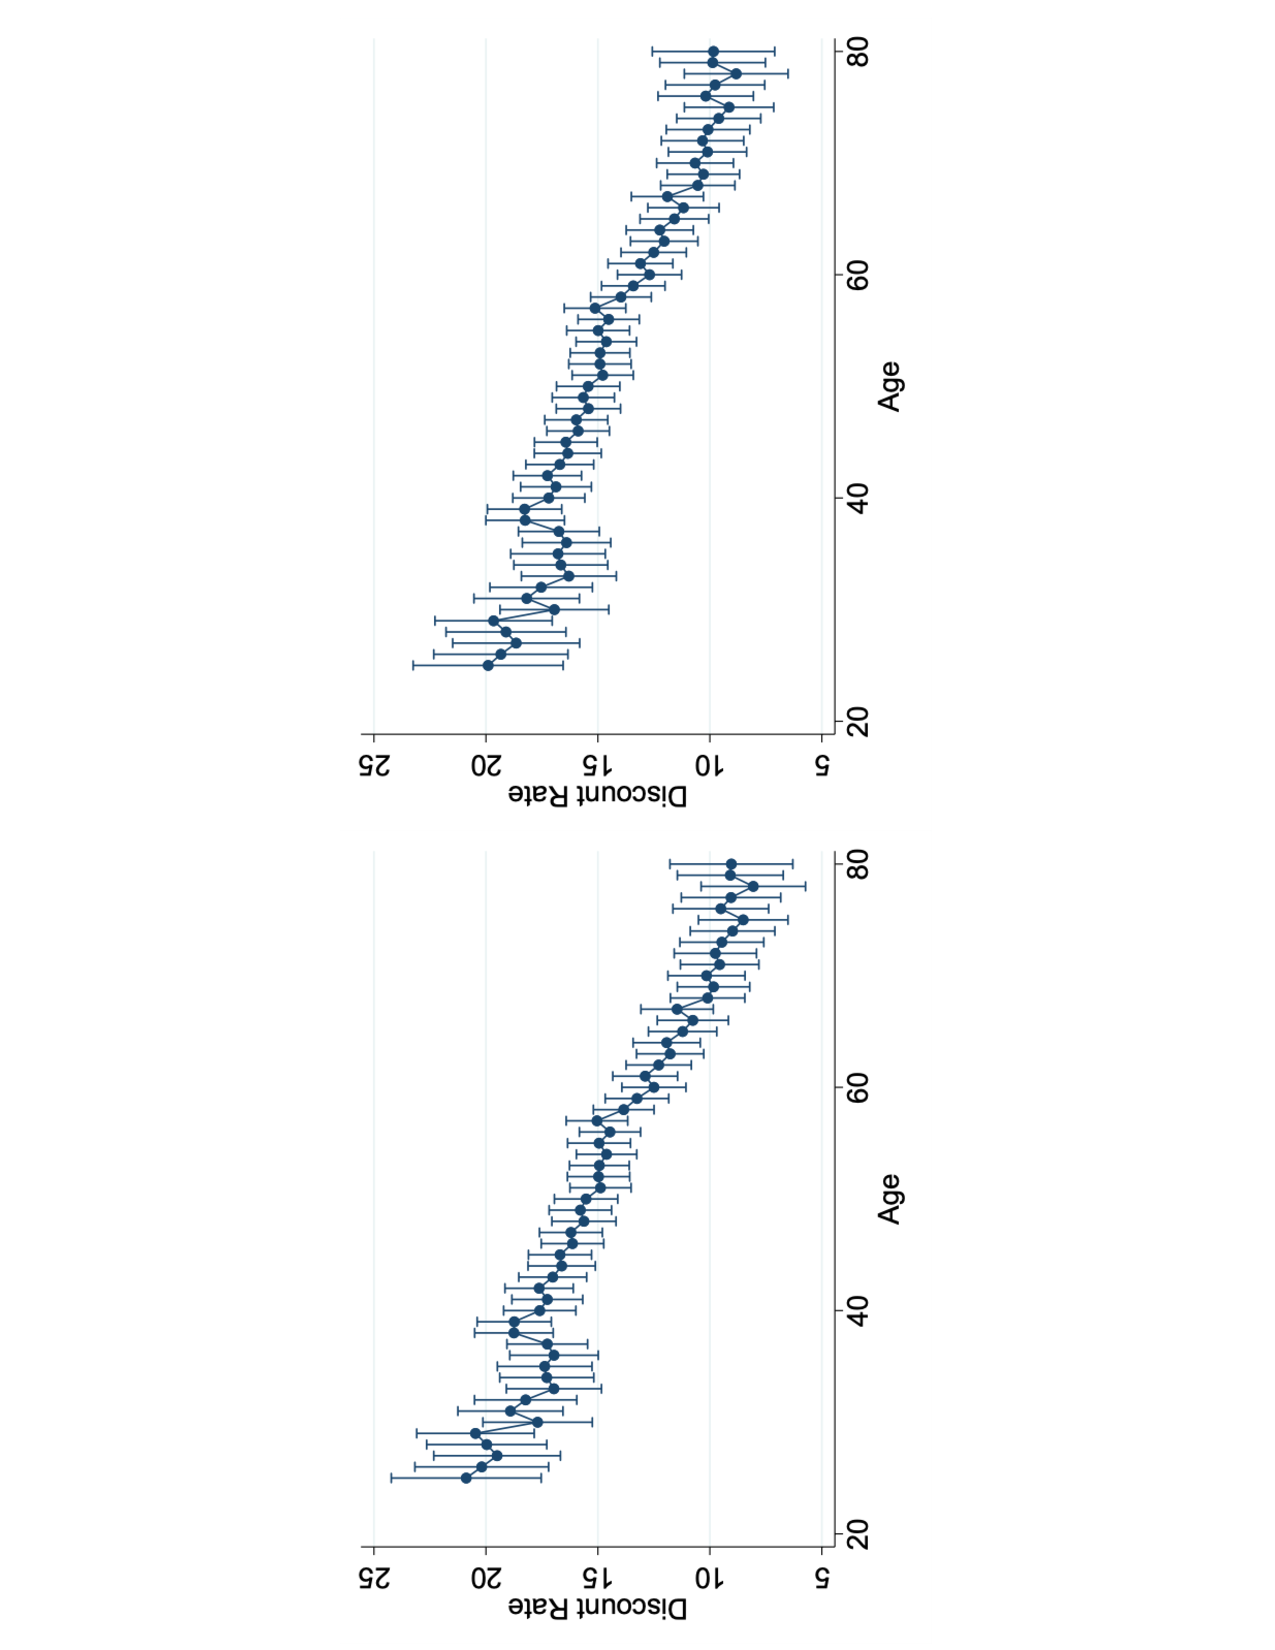
\includegraphics[scale=.35, angle=-90, trim= 5cm  0cm 5cm 0cm,clip]{fig/age_dependent_discount_rates.pdf}
}



\item[working period] age or working period out of the total number of working periods. People are initialized with a random working period between 0 and the number of working period (40).
\end{description}

\subsubsection{Firm}
We use a Cobb-Douglas production function $Y=A_F k_F^\alpha  n_F^\beta$ with diminishing returns to scale. 

\begin{description}

\item [scale factor $A_F$] = 53.34721 (computed in production appendix.)

\item  [alpha\_firm  $\mathbf{\alpha_F}$] = 0.18 (typically 0.2 in macro models, but empirically values are lower, and lower values leave room for agglomeration effects),  for a single firm with a production function $Y_{Fi}=A_F K_i^{\alpha_F }L^{\beta_F}_i$ (empirical range =)\footnote{According to Vollrath,``In the U.S. from 1948-1995 the capital elasticity bounds were 0.18-0.33, and rose to 0.21-0.39 in 1995-2018.''\cite{vollrathElasticityAggregateOutput2021} Vollrath also found that the capital elasticity in the private business sector is 0.09-0.28 from 1948-1995, and 0.16-0.33 from 1995-2018, and it is lower if intellectual capital is excluded.}

\item  [beta\_firm $\mathbf{\beta_F}$] = 0.72 (typically 0.8 in macro models, but empirically values are lower, and lower values leave room for agglomeration effects). Also called the elasticity of output with respect to labour for a single firm. (empirical)\footnote{Douglas  obtained a result for the exponent of labour of 0.75—which was subsequently confirmed by the National Bureau of Economic Research to be 0.741. Lower values  are associated with stronger decreasing returns to scale for the firm in our model.} 
\item [initial workforce of a standard rural firm] $n_R=100$. This is constant in our modeling. 

\item [initial workforce of a standard urban firm] $n_0=n$.  The urban firm workforce will evolve over time: $n_{Ut}$. 

\item [price of output] = 1. (If you wanted to be able to vary this, you would put a price parameter in front the % of marginal products. 
\gls{marginal product of labour}. %pMPL)

\item [firm cost of capital] $r = 0.05$ or 5\%.
\item[wage premium ratio $p$] is the 
\item [initial wage premium]  
\[\omega_0 = p \psi\] 
where $p$ is the wage premium ratio. If it is 0.2, then $\omega_0= 0.2*\psi =\$8000$ and the urban wage is 1.2 times the rural wage.

\item [wage adjustment coefficient for new workers ] $adj^{new}_\omega=.5$

\item [wage adjustment coefficient for existing workers] $adj^{existing}_\omega=.5$
\end{description}
    

\subsubsection{Bank} % and mortgage parameters
\begin{description}
\item [mortgage period]  mortgage\_period ($\mathbb{T}$)
\item [cost of capital for the bank] r\_prime. The bank's interest rate, $r$, is just the bank rate (r\_prime) set by the Bank of Canada.  
% The bank's interest rate, $r$, is just the bank rate (prime rate? set by the Bank of Canada. Exogenous. Just assign  a value like 4\%.

\item [r\_margin = 2\%] The bank's required markup on funds when it lends.  

\item [r\_target] reference rate that the bank demands on loans on 
$ r^{target}= r^{prime} +r^{margin}$ ? 

\item[lending rate/borrowing rate $r_i$]  
\[r_i=r^{prime} + r^{target} + \mathrm{individual\_wealth\_adjustment}\]

\item [{ability to carry a mortgage}] the share of income that can be used to cover mortgage interest. This represents the rule of thumb for households that they should not spend more than 25\% or 30\% of their income on on housing. We use 0.28.

\item [\gls{maximum mortgage share} of price] parameter in calculation of $m_i$. Specific to the functional form used. Set at 0.9. Based on stylized facts from the literature.  % No empirical estimates are available.
\item[wealth sensitivity] of maximum mortgage share of price. This is a parameter in the calculation of $m_i$. It is specific to the functional form used. Set at 0.1. The choice of a function is based on stylized facts from the literature.  %No empirical estimates are available. 
Used in Equation~\ref{eqn-wealth-based-mortgage}.

\item [$K$ the wealth sensitivity of the borrowing rate for those purchasing homes]
\end{description}




% \subsection{Initial values for endogenous variables} \label{sec-init-value-list}



\subsection{Housing Market}
\begin{description}
\item [initial market rent] 
Initial rent cost for tenants  $\mathcal{R}_{M, 0}= \mathcal{R}_W$.

\item [Initial market price] 
$P_0= P_W=\frac{\mathcal{R}_W }{r}$,  
\end{description}


\subsection{Net warranted price} \label{section-warranted-price}
We use the net warranted price to approximate the initial value of the market price in our computational model. 
The economically \gls{warranted price}, for an agent, borrowing money to purchase a property, is the present discounted value of the flow of service net of costs. The present discounted value of the infinite stream of net rents is:
\begin{equation}
P_W=\frac{\mathcal{R}_N}{r},  
\label{eqn-price-warranted}
\end{equation}
where $\mathcal{R}_N$ is the net value of annual rents, and $r$ is the interest rate.  
%In a market in equilibrium, the warranted price should approximate the sale price, of a unit of housing with land, in the absence of potential capital gains and expected changes in its components.  We use the  present discounted value of net warranted rents to 


\subsection{Person}
\begin{description}
\item[savings] $age_i*savings\_rate*\psi$
\item[personal wealth] $W_{i0}= savings + warranted\_price $
\item[average wealth] $\bar W_{0}= \sum_i W_i$
\item[Subjective discounting] The discount factor gives the present value of one dollar received at a particular point in the future, given the date of receipt and the discount rate.

{discount rate vs discount factor}

We have called the  discount rate is $\delta$ (it might be better to call it $rho$.) We assumed it equal to $r_i$. This is a pretty strong assumption.

The discount \textbf{factor} $\delta(t)$ is a function of $\delta_i$ and the time until the event, $t$
% delta(0)=1  delta (1)= 1/(1+r) 
\[\delta(t)=\left(\frac{1}{1+\delta}\right)^t\]
\[delta(T)=  (1/(1+\delta))^T\]   

\end{description}



(insert tables? from the CHSP?) as in from model chapter 'According to the Canada Housing Statistics Program (CHSP), first-time home buyers require a combination of sufficient income and savings in order to enter the housing market'

TODO MOVE TO WHEREVER WE PUT EMPIRICAL VALUES INFORMING PARAMETER SETTING - APPENDIX? According to Statistics Canada's Survey of Household Spending for 2019, \cite{statisticscanadaSurveyHouseholdSpending2021} homeowners with mortgages allocated about 29\% of their total  spending to shelter costs (\$30,734), with mortgage payments (\$16,959) accounting for more than half of this total.

The median after-tax income of Canadian families and unattached individuals was \$66,800 in 2020 according to Statistics Canada. %'s 
%\href{https://www150.statcan.gc.ca/n1/daily-quotidien/220323/dq220323a-eng.htm}{Canadian Income Survey, 2020}.  \href{https://www150.statcan.gc.ca/t1/tbl1/en/tv.action?pid=1110005501}
% Data released in 2020 by Statistics Canada indicates that t
 The top 1\% of reporting Canadians made, on average, around \$512,000 in a single year \cite{WEB_model-stats-can-canadian-incomes}. % \href{https://www150.statcan.gc.ca/n1/daily-quotidien/201222/dq201222b-eng.htm}{Survey of Financial Security, 2019}.
 %A study by Statistics Canada found that t
  %\href{https://www150.statcan.gc.ca/t1/tbl1/en/tv.action?pid=1110005501}{High income tax filers in Canada}


(TODO MOVE TO APPENDIX WHERE WE INTRODUCE VALUES OT SET PARAMETERS Wealth, $\bar W$, limits borrowing amounts and interest rates in Equation \ref{eqn-wealth-based-mortgage}. The median net worth of Canadian households is \$329,900, while the average net worth in Canada is \$738,200 \cite{WEB-model-stats-can-median-net-worth}.)

The nature of the constraint is
Figure~\ref{fig-borrowing-ratio} illustrates the model rising asymptotically to a maximum mortgage share of 0.9. % The function here rises asymptotically to 0.9. 
The borrowing ratio for the median wealth holder is perhaps 0.8. The institutional investor in our model has a borrowing ratio close to or at the maximum since it is not asset constrained. While and the general relationship we describe here is clearly established empirically \cite{GET_SOURCE}, the functional form and parameter values are somewhat arbitrary. %we have not found precise estimates or parameters. 


(TODO MOVE TO PARAMETER SETTING SECTION Many personal finance experts recommend total housing costs account for less than  28\% of \textbf{gross} household income, so we use value 0.28 as an estimate of $i$'s annual carrying capacity  $\mathbb{C}$ in Equation \ref{eqn-income-based-mortgage}.)
